\documentclass[letterpaper,12pt]{article}
\usepackage[margin=2cm]{geometry}

\usepackage{graphicx}

\title{\textbf{RTES Lab4 Writeup}}
\author{Mengwen He}

\begin{document}

\maketitle

\begin{enumerate}
	\item When and why would you want to compile your kernel in NO\_HZ configuration?\\
	\textbf{Answer:}\\
	When the macro HZ being set at compile time and varying between around 100 to 1500, it enables a timer tick to interrupt the kernel HZ times per second. Therefore, when we want a tickless kernel, we need to compile the kernel in NO\_HZ configuration. The reason is that running without a timer tick means the kernel does less work when idle and can potentially save power because it does not have to wake up regularly just to service the timer.
	
	\item What kernel subsystem decides which sleep state the processor enters and what parameters does it use to make the decision?\\
	\textbf{Answer:}\\
	The kernel cpuidle subsystem decides which sleep state the processor enters. The kernel uses the struct cpuidle\_state to make the decision.
	
	\item What are advantages and disadvantages of the wake locks solution adopted by the Android fork of the Linux kernel?\\
	\textbf{Answer:}\\
	Wake locks are power-managing software mechanisms, which make sure that the Android device doesn't go into deep sleep. The advantage is that the wake locks can keep the cpu to run some background applications. The disadvantage is that the abuse of wake locks leads to anomalous battery drain.
	
	\item In the kernel you are working on for Nexus 7, does voltage change when frequency changes?\\
	\textbf{Answer:}\\
	Yes, the voltage changes when the frequency changes because we find the DVFS in the Nexus 7's kernel cpufreq\_governor.
	
	\item In ARM architecture, what instruction can be used to enter a low-power processor state?\\
	\textbf{Answer:}\\
	The arm\_enter\_idle\_state or cpuidle\_generic\_enter function can be used to enter a low-power state.
		
\end{enumerate}

	\begin{figure}
		\centering
		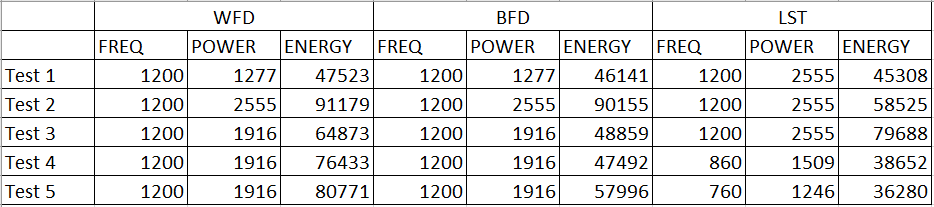
\includegraphics[width=0.8\textwidth]{./img/T1}\\
		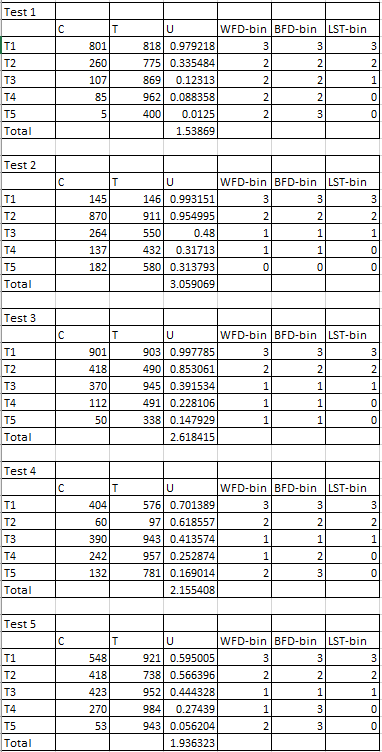
\includegraphics[width=0.4\textwidth]{./img/T2}\\
	\end{figure}
	\newpage
	\begin{figure}
		\centering
		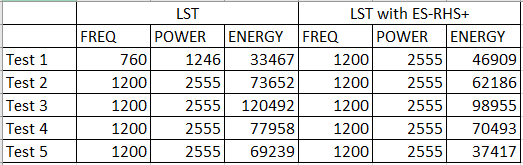
\includegraphics[width=0.8\textwidth]{./img/T3}\\
		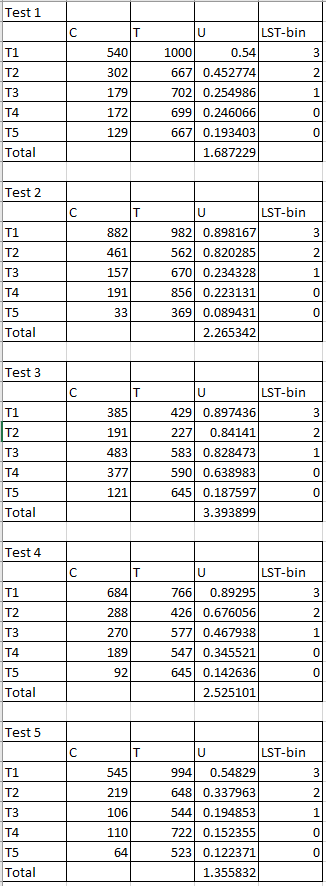
\includegraphics[width=0.35\textwidth]{./img/T4}\\
	\end{figure}
	\newpage
	\begin{figure}
		\centering
		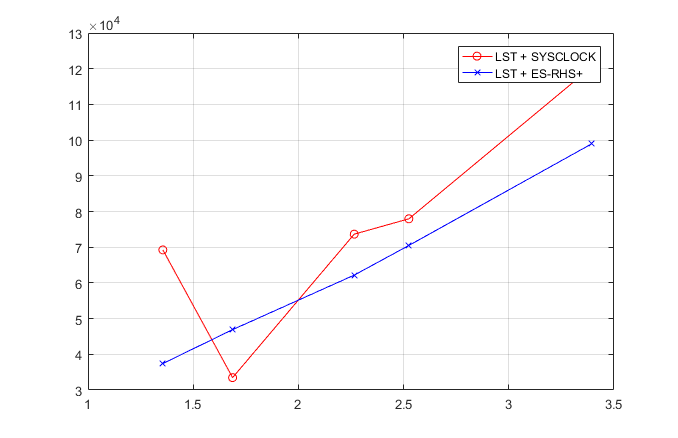
\includegraphics[width=0.9\textwidth]{./img/result}\\
	\end{figure}

\end{document}